\documentclass[border=2pt]{standalone}
%%
%% Use this file to regenerate tikz diagrams by building the pdf and converting to SVG.
%%
%%     lualatex -halt-on-error -interaction=batchmode Rewards-Diagram.tex
%%     dvisvgm --pdf --page=1 -n -a -o Rewards-Diagram.svg Rewards-Diagram.pdf
%%     cp Rewards-Diagram.svg ../md/common/src/img/
%%
%% (`--pdf` tells `dvisvgm` to read the PDF, `-n` outlines text so the svg file is
%% self-contained, `-a` preserves transparency)
%%
%% Use the resulting .svg file in a Markdown file as follows:
%%
%%    ![Rewards-Diagram](img/Rewards-Diagram.svg)
%%
\usepackage{pgfplots}
\usepackage[tikz]{bclogo}
\usepackage{tikz-cd}
\usetikzlibrary{ arrows.meta
               , backgrounds
               , calc
               , decorations.pathreplacing
               , fit
               , positioning
               , shadows
               , shapes.geometric
               , shapes.misc
               }
\usepackage[dvipsnames]{xcolor}
\usepackage{caption}

\begin{document}
    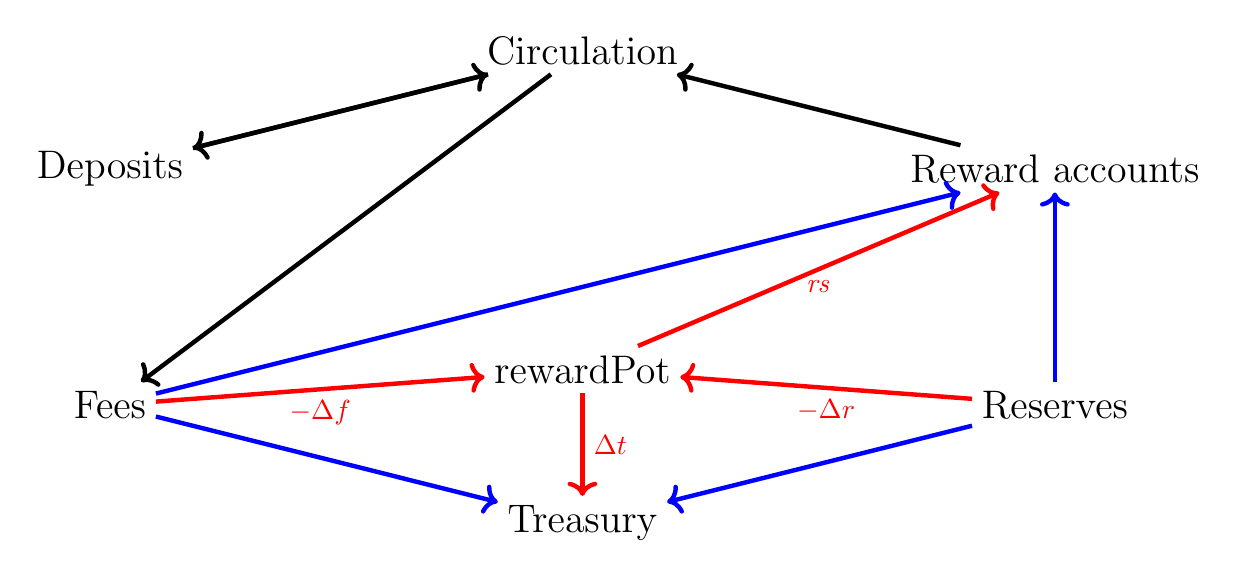
\begin{tikzpicture}
      [ x=30mm, y=30mm
      , direct/.style={black, draw}
      , implied/.style={blue, draw}
      , toTotPot/.style={red, draw}
      ]
    \node (C) at (3,2.5) {\Large Circulation};
    \node (R) at (5, 1) {\Large Reserves};
    \node (D) at (1, 2) {\Large Deposits};
    \node (FR) at (1,1) {\Large Fees};
    \node (RA) at (5, 2) {\Large Reward accounts};
    \node (T) at (3,0.5) {\Large Treasury};

    \draw[->, direct, ultra thick]
    (C) edge (D)
    (C) edge (FR)

    (D) edge (C)

    (RA) edge (C);

    \draw[->, implied, ultra thick]
    (FR) edge (T)
    (FR) edge (RA)

    (R) edge (T)
    (R) edge (RA);

    \node (TP) at (3, 1.15) {\Large rewardPot};

    \draw[->, toTotPot, ultra thick]
    (FR) edge node[below] {$-\Delta f$} (TP)
    (R)  edge node[below] {$-\Delta r$} (TP)

    (TP) edge node[below] {\textit{rs}} (RA)
    (TP) edge node[right] {$\Delta t$} (T);
    \end{tikzpicture}

\end{document}
